\chapter{Biología de la conservación}\label{ch:b3:conservation-biology}

En 1813 Audubon vio pasar sobre Kentucky durante tres días una bandada
de palomas migratorias que oscurecía el cielo; había quizá cinco mil
millones de ellas, la cuarta parte de todas las aves de América del
Norte. El 1 de septiembre de 1914 murió la última, una hembra llamada
Martha, en el zoo de Cincinnati. La especie no era rara cuando empezó
su declive; se la cosechaba por vagones, se talaban sus bosques, y un
ave que solo criaba en colonias inmensas no podía criar una vez que las
colonias se habían raleado por debajo de un tamaño que nadie midió. En
1995 el kakapo, un loro nocturno no volador de Nueva Zelanda, había
bajado a cincuenta y un ejemplares; desde entonces todos han sido
bautizados, pesados, equipados con un transmisor y, en el momento
oportuno, alimentados con un suplemento, y ya son doscientos cincuenta.
Ese mismo año se soltaron treinta y un lobos grises en Yellowstone,
setenta años después de que se abatiera a la última manada nativa; en
dos décadas los uapitíes se habían desplazado, los sauces habían vuelto
a las riberas y los castores con ellos. La biología de la conservación
es la aplicación de la genética de poblaciones, la ecología y el
comportamiento de este libro a una sola pregunta práctica ---cómo
impedir que desaparezcan las especies--- y su aritmética es la
aritmética de los números pequeños.

\section{Por qué mueren las poblaciones pequeñas}

\begin{definition}[Los riesgos de la pequeñez]\label{def:b3:conservation-biology:small}
\index{estocasticidad demográfica}\index{estocasticidad ambiental}\index{efecto Allee}\index{vórtice de extinción}\index{población mínima viable}
Una población grande declina cuando su \omterm{prop:b3:stem-cells:gompertz}{tasa de mortalidad} supera a la
de natalidad; una pequeña puede desaparecer sin cambio alguno en
ninguna de las dos. La \emph{estocasticidad demográfica} es la
posibilidad de que, entre unos pocos individuos, mueran por azar más de
los que nacen, o de que todos los supervivientes sean machos: importa
por debajo de unas pocas docenas. La \emph{estocasticidad ambiental}
---un mal invierno, una sequía, una enfermedad--- golpea a la vez a
todos los individuos, y una población de unos pocos cientos que una
grande capearía puede quedar aniquilada; las \emph{catástrofes} son su
cola. El \emph{efecto Allee} hace caer la tasa de crecimiento per
cápita a densidad baja ---no se encuentran parejas, las especies
coloniales no pueden anidar, las manadas no pueden defender a sus
crías, las bandadas de la paloma migratoria no podían saturar a los
depredadores que se llevaban a sus pichones---, de modo que por debajo
de una densidad umbral la población declina por sí sola hacia cero. Y
por debajo de unos pocos cientos, los procesos genéticos de la sección
siguiente reducen la eficacia generación tras generación. Todo esto se
alimenta entre sí: una población más pequeña pierde variación, se
vuelve menos fértil, encoge, tiene más probabilidades de recibir un
golpe del azar y pierde más ---el \emph{vórtice de extinción} (Gilpin y
Soulé, 1986). Una \emph{población mínima viable} es el tamaño por
encima del cual la probabilidad de extinción en un horizonte dado
(pongamos el \qty{5}{\%} en un siglo) resulta aceptable; depende de la
biología de la especie y de cuán variable sea su ambiente, y suele
estar en los miles.
\end{definition}

\begin{omfigure}
\begin{tikzpicture}[every node/.style={font=\scriptsize}, >=stealth]
  \node[draw, thick, rounded corners, fill=omThm!20, align=center] (small) at (0,0) {la población\\se vuelve pequeña};
  \node[draw, thick, rounded corners, fill=omDef!20, align=center] (drift) at (3.4,1.6) {deriva y endogamia:\\variación perdida, $F$ sube};
  \node[draw, thick, rounded corners, fill=omDef!20, align=center] (fit) at (6.8,0) {la eficacia cae:\\menos crías, más\\enfermedad};
  \node[draw, thick, rounded corners, fill=omDef!20, align=center] (chance) at (3.4,-1.6) {el azar demográfico y ambiental\\muerde más fuerte};
  \node[draw, thick, rounded corners, fill=omProp!25, align=center] (allee) at (9.9,0) {efecto Allee:\\crecimiento negativo};
  \draw[->, very thick] (small) -- (drift); \draw[->, very thick] (drift) -- (fit); \draw[->, very thick] (fit) -- (chance); \draw[->, very thick] (chance) -- (small);
  \draw[->, thick, omProp!80!black] (fit) -- (allee); \draw[->, thick, omProp!80!black] (allee.south) .. controls (9.9,-3) and (0,-3.4) .. (small.south);
  \node[align=center, font=\tiny] at (3.4,0) {el vórtice de extinción:\\cada vuelta encoge la\\población y acelera la siguiente};
  \node[left, align=right, font=\tiny] at (-1.7,1.5) {pérdida de hábitat, caza,\\depredadores, enfermedad:\\empujan a la población};
  \draw[->, thick, gray] (-1.6,1.2) -- (small.north west);
\end{tikzpicture}

{\small El \omterm{def:b3:conservation-biology:small}{vórtice de extinción}. Un golpe externo vuelve pequeña a una
población; la pequeñez pierde entonces variación, baja la eficacia,
expone a la población al azar y la vuelve más pequeña todavía. La tarea
de la conservación es romper el bucle antes de que se cierre.}
\end{omfigure}

\begin{theorem}[El tamaño efectivo de población]\label{thm:b3:conservation-biology:ne}
\index{tamaño efectivo de población}\index{proporción de sexos}\index{media armónica}\index{coeficiente de endogamia}\index{heterocigosidad}
El ritmo al que una población pierde variación y acumula endogamia no
lo gobierna su tamaño censal $N$, sino su \emph{tamaño efectivo}
$N_{e}$: el tamaño de una población ideal ---constante, de apareamiento
aleatorio, con \omterm{thm:b3:conservation-biology:ne}{proporción de sexos} igual y tamaños de familia de
Poisson--- que perdería heterocigosidad al mismo ritmo. Tres
desviaciones del ideal lo rebajan. Una \omterm{thm:b3:conservation-biology:ne}{proporción de sexos} desigual, con
$N_{m}$ machos y $N_{f}$ hembras reproductores:
\[
N_{e} = \frac{4N_{m}N_{f}}{N_{m} + N_{f}} ;
\]
un macho y cien hembras dan $N_{e} \approx 4$. Un tamaño fluctuante a lo
largo de $t$ generaciones: $N_{e}$ es la \emph{\omterm{thm:b3:conservation-biology:ne}{media armónica}} de los
tamaños de las generaciones, $1/N_{e} = (1/t)\sum 1/N_{i}$, dominada por
el menor ---una población de mil que en algún momento pasó por diez
tiene un $N_{e}$ cercano a cien en ese tramo. Y una varianza del tamaño
de familia por encima de la de Poisson lo rebaja más. En una población
de tamaño efectivo $N_{e}$, el \emph{\omterm{thm:b3:conservation-biology:ne}{coeficiente de endogamia}} $F$ ---la
probabilidad de que los dos alelos de un locus de un individuo sean
copias de un mismo alelo ancestral--- sube $1/2N_{e}$ por generación,
\[
F_{t} = 1 - \Bigl(1 - \frac{1}{2N_{e}}\Bigr)^{t} \approx \frac{t}{2N_{e}},
\qquad H_{t} = H_{0}\Bigl(1 - \frac{1}{2N_{e}}\Bigr)^{t} ,
\]
y la \emph{heterocigosidad} $H$ decae al mismo ritmo. La regla práctica
de Franklin, ``50/500'': $N_{e} \ge 50$ mantiene la endogamia por debajo
del \qty{1}{\%} por generación, el ritmo que toleran los criadores de
animales; $N_{e} \ge
500$ deja que la mutación reponga la variación que retira la deriva.
Como $N_{e}$ suele ser la décima parte del tamaño censal, la regla pide
poblaciones de quinientos a cinco mil.
\end{theorem}
\begin{proof}
Dos gametos tomados al azar de la población son copias del mismo alelo
parental con probabilidad $1/2N$ en la población ideal, que es el
incremento de $F$; la heterocigosidad es $1 - F$ reescalada, de modo que
cada generación la multiplica por $(1 - 1/2N_{e})$, lo que da el
decaimiento exponencial y, para $t \ll N_{e}$, la subida lineal de $F$.
\omterm{thm:b3:conservation-biology:ne}{Proporción de sexos}: la mitad de los genes viene de cada sexo, de modo
que la probabilidad de que dos gametos compartan un alelo parental es
$\tfrac{1}{4}\cdot\tfrac{1}{2N_{m}} +
\tfrac{1}{4}\cdot\tfrac{1}{2N_{f}}$ (una cuarta parte de los pares son
ambos paternos y otra cuarta parte ambos maternos); igualando esto a
$1/2N_{e}$ resulta $1/N_{e} = 1/(4N_{m}) + 1/(4N_{f})$, la fórmula.
Fluctuación: la heterocigosidad tras $t$ generaciones es
$H_{0}\prod(1 - 1/2N_{i})
\approx H_{0}\exp(-\sum 1/2N_{i})$, igual a $H_{0}\exp(-t/2N_{e})$
cuando $1/N_{e}$ es la media de los $1/N_{i}$. La endogamia baja la
eficacia porque expone como homocigotos los alelos recesivos deletéreos
---la \emph{depresión por endogamia}, una caída de un pequeño
porcentaje en supervivencia o fecundidad por cada \qty{10}{\%} de $F$ en
la mayoría de las especies de cruzamiento externo.
\end{proof}

\begin{omfigure}
\begin{tikzpicture}
\begin{axis}[
  width=0.46\linewidth, height=5.2cm,
  axis x line=bottom, axis y line=left,
  xmin=0, xmax=1, ymin=0, ymax=1.05,
  xlabel={fracción de reproductores que son machos}, ylabel={$N_{e}/N$},
  xlabel style={font=\small, at={(axis description cs:0.5,-0.12)}, anchor=north}, ylabel style={font=\small},
  tick label style={font=\small}, xtick={0,0.1,0.5,0.9,1}, ytick={0.36,1},
  clip=false,
]
\addplot[very thick, omDef, domain=0.005:0.995, samples=100] {4*x*(1-x)};
\draw[dashed, gray] (axis cs:0.1,0) -- (axis cs:0.1,0.36) -- (axis cs:0,0.36);
\node[font=\scriptsize, omDef, anchor=south] at (axis cs:0.5,1.0) {sexos iguales: $N_{e} = N$};
\node[font=\scriptsize, anchor=west, align=left] at (axis cs:0.12,0.2) {un macho de cada diez\\se reproduce: $N_{e} = 0.36N$};
\end{axis}
\begin{axis}[
  at={(0.5\linewidth,0)}, anchor=south west,
  width=0.46\linewidth, height=5.2cm,
  axis x line=bottom, axis y line=left,
  xmin=0, xmax=100, ymin=0, ymax=1.05,
  xlabel={generaciones}, ylabel={heterocigosidad $H_{t}/H_{0}$},
  xlabel style={font=\small, at={(axis description cs:0.5,-0.12)}, anchor=north}, ylabel style={font=\small},
  tick label style={font=\small}, xtick={0,25,50,75,100}, ytick={0.37,0.6,0.9,1},
  yticklabels={0.37,0.6,0.9,1},
  clip=false,
]
\addplot[very thick, omThm, domain=0:100, samples=60] {(1-1/20)^x};
\addplot[very thick, omMeth!70!black, domain=0:100, samples=60] {(1-1/100)^x};
\addplot[very thick, omDef, domain=0:100, samples=60] {(1-1/1000)^x};
\node[font=\scriptsize, omThm, anchor=north west] at (axis cs:12,0.55) {$N_{e} = 10$};
\node[font=\scriptsize, omMeth!70!black, anchor=south west] at (axis cs:50,0.62) {$N_{e} = 50$};
\node[font=\scriptsize, omDef, anchor=south west] at (axis cs:60,0.95) {$N_{e} = 500$};
\end{axis}
\end{tikzpicture}

{\small Izquierda: cómo una \omterm{thm:b3:conservation-biology:ne}{proporción de sexos} sesgada encoge el
tamaño efectivo ---una especie de harén con una décima parte de los
machos reproduciéndose tiene un $N_{e}$ de un tercio de su censo.
Derecha: la heterocigosidad decayendo en $(1 - 1/2N_{e})$ por generación
---una población de diez pierde casi toda su variación en un siglo, y
una de quinientos casi nada.}
\end{omfigure}

\begin{proof}[Evidencia]
La pantera de Florida, reducida a unos veinticinco animales en los años
noventa, mostraba colas dobladas, testículos no descendidos, defectos
cardíacos y un esperma del que el \qty{90}{\%} era anómalo ---la
depresión por endogamia hecha visible; ocho hembras introducidas desde
Texas en 1995 (un \emph{rescate genético}) triplicaron la población y
los defectos retrocedieron. Los lobos de Isle Royale, fundados por una
pareja en 1949 y aislados, declinaron hasta dos individuos
groseramente endogámicos en 2018, con deformidades de la columna en la
mayoría de los esqueletos examinados. El gallo de las praderas grande
de Illinois cayó de miles a cincuenta, y su tasa de eclosión del
\qty{93}{\%} al \qty{56}{\%}, y se recuperó tras traer aves de otros
estados. Las pieles de museo y el ADN antiguo permiten medir
directamente en cada caso la pérdida de heterocigosidad frente a la
población anterior al declive.
\end{proof}

\begin{omfigure}
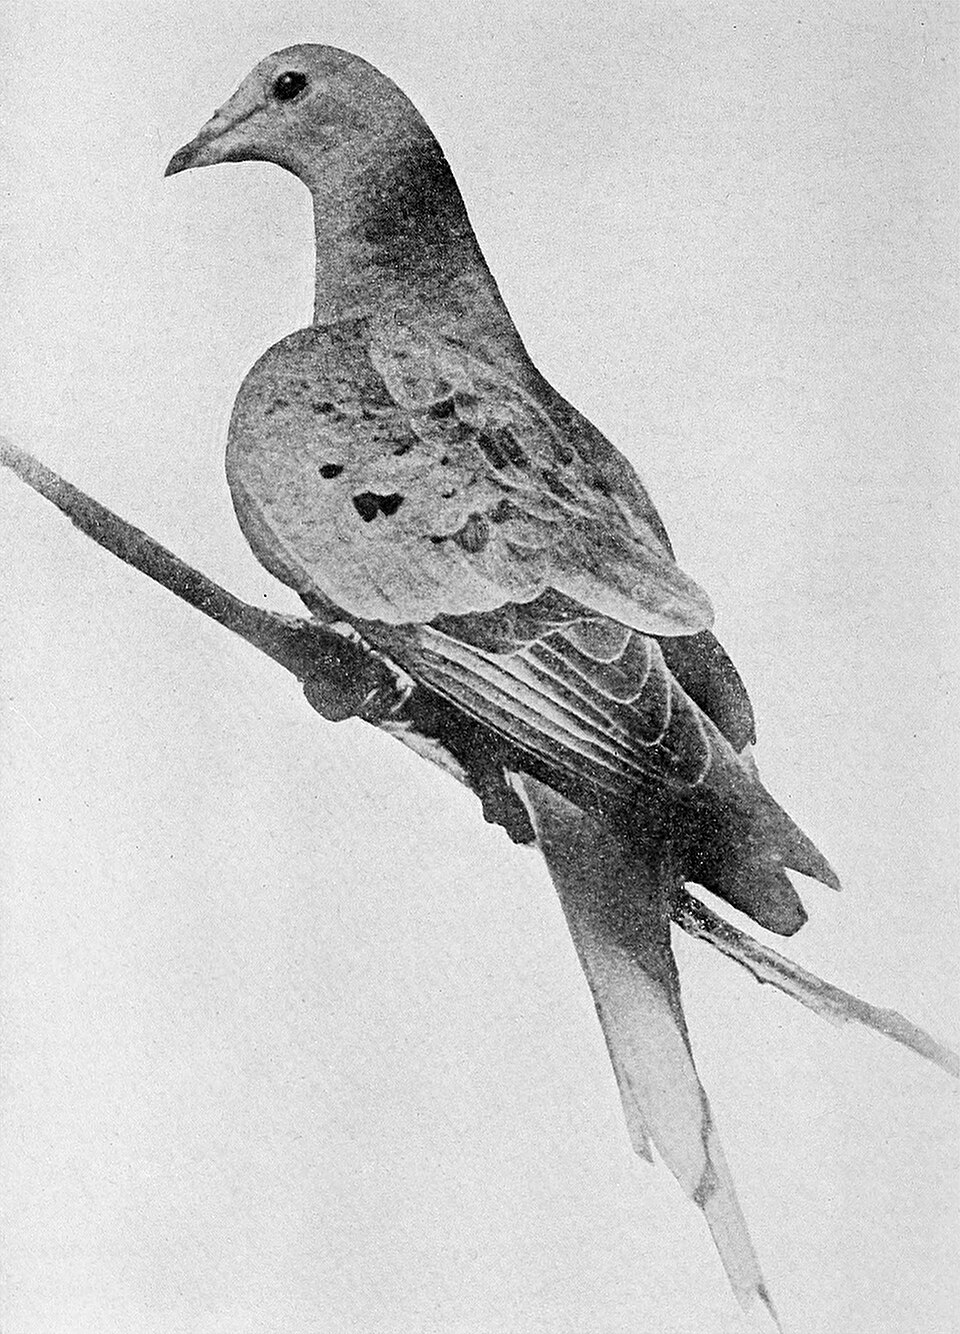
\includegraphics[width=0.4\linewidth]{images/book5/martha.jpg}\hspace{0.04\linewidth}
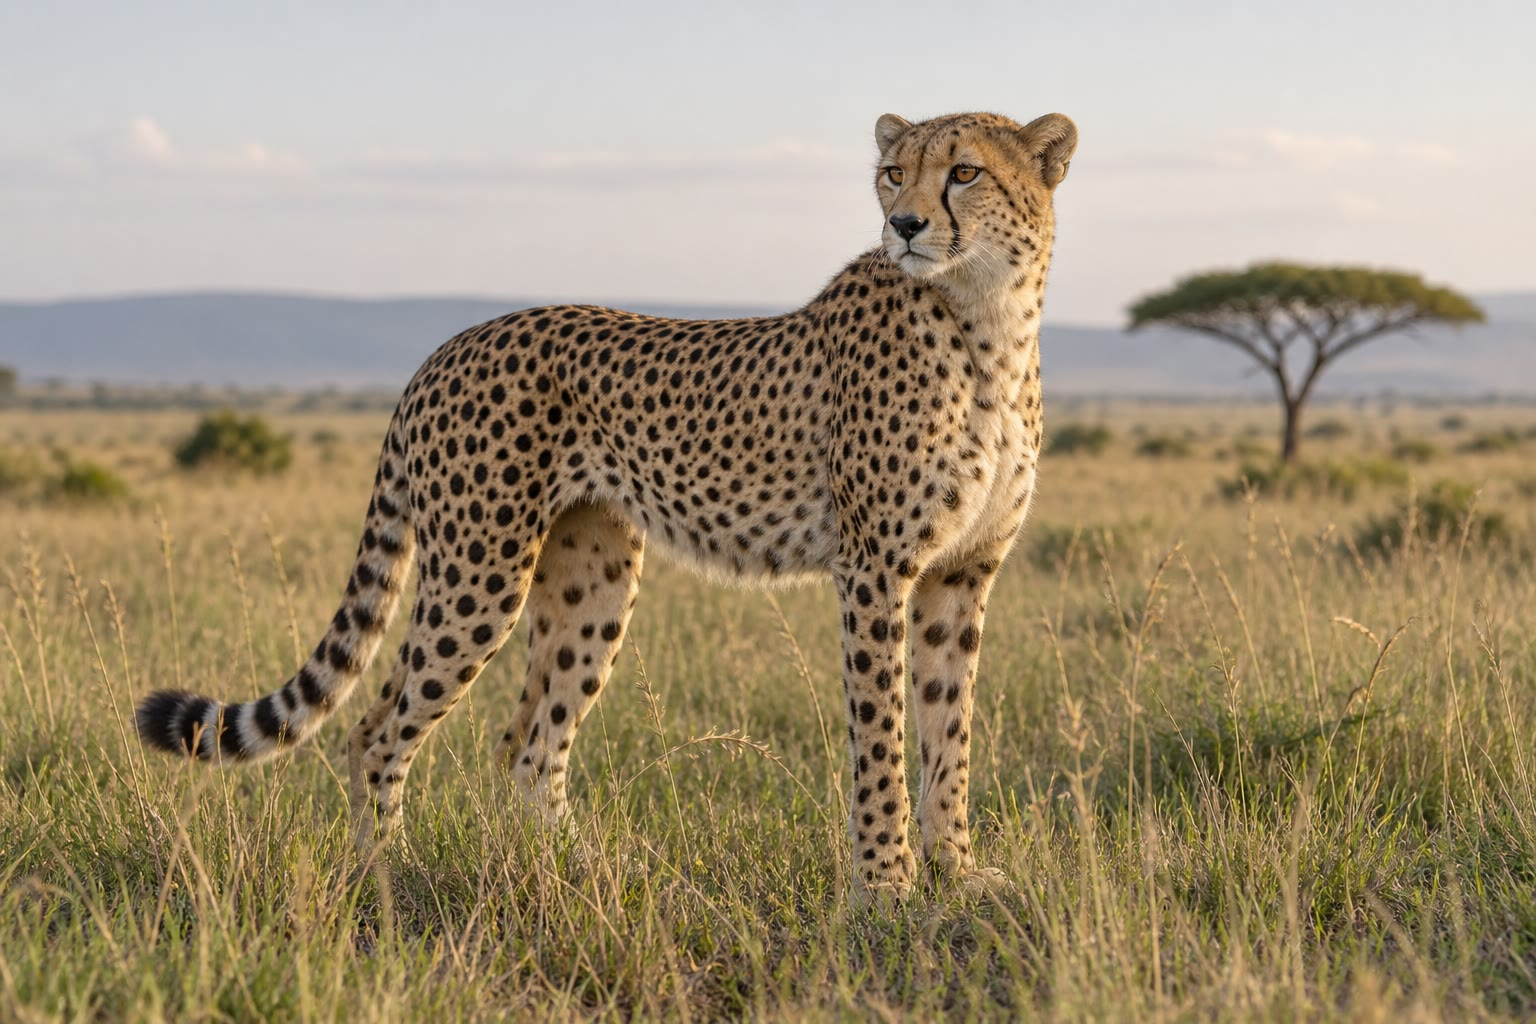
\includegraphics[width=0.52\linewidth]{images/book5/ai/b5-27-cheetah.jpg}

{\small Izquierda: Martha, la última paloma migratoria, fotografiada en
el zoo de Cincinnati en 1912; la especie se había contado por miles de
millones dentro de la memoria viva (fotografía de Enno Meyer, dominio
público). Derecha: un guepardo ---una especie que atravesó un cuello de
botella hace unos diez mil años y cuyos individuos son tan parecidos
que los injertos de piel entre animales sin parentesco no se rechazan.}
\end{omfigure}

\section{El hábitat: cuánto y de qué forma}

\begin{proposition}[Especies y área]\label{prop:b3:conservation-biology:area}
\index{relación especies--área}\index{fragmentación del hábitat}\index{biogeografía insular}\index{corredor}\index{debate SLOSS}\index{efecto de borde}
En las islas, y en los fragmentos de hábitat que se comportan como
islas, el número de especies $S$ sube con el área $A$ como una ley
potencial,
\[
S = c\,A^{z}, \qquad z \approx 0.15\text{--}0.35,
\]
la \emph{\omterm{prop:b3:conservation-biology:area}{relación especies--área}} (Arrhenius, 1921; la \omterm{prop:b3:conservation-biology:area}{biogeografía
insular} de MacArthur y Wilson, 1967, la explicó como un equilibrio
entre inmigración y extinción, siendo la extinción más rápida en las
islas pequeñas). Con $z = 0.25$, perder el \qty{90}{\%} del área de un
hábitat acaba costando el $1 - 0.1^{0.25} = \qty{44}{\%}$ de sus
especies; perder la mitad cuesta el \qty{16}{\%}. La pérdida no es
inmediata ---una \emph{deuda de extinción} se paga a lo largo de
décadas, a medida que menguan las poblaciones demasiado pequeñas para
sus fragmentos--- y la \emph{fragmentación} de un área fija en trozos
añade pérdidas propias: cada fragmento alberga una población menor, los
\emph{\omterm{prop:b3:conservation-biology:area}{efectos de borde}} (viento, calor, depredadores, malas hierbas)
penetran cientos de metros en el bosque, y las especies que necesitan el
interior pierden más de lo que el área explica. Que salve más especies
una sola reserva grande o varias pequeñas de la misma área total (el
debate \emph{SLOSS}) depende de las especies: la grande alberga
poblaciones mayores y hábitat interior, y las pequeñas reparten el
riesgo de una catástrofe y muestrean más tipos de hábitat. Los
\emph{corredores} que conectan fragmentos dejan moverse entre ellos a
individuos y genes, y convierten poblaciones aisladas en una
metapoblación cuyas partes pueden recolonizarse tras una extinción
local y rescatarse de la endogamia ---por lo que el terreno situado
entre las reservas ha pasado a preocupar tanto como las reservas.
\end{proposition}
\begin{proof}
La ley potencial es empírica, ajustada en ejes logarítmicos a
archipiélagos, lagos, cumbres y fragmentos de bosque del mundo entero;
el valor de $z$ es menor para trozos de un continente (la inmigración
mantiene presentes a las especies) y mayor para las islas verdaderas.
La pérdida relativa se sigue directamente: $S'/S = (A'/A)^{z}$. El
mecanismo de la \omterm{prop:b3:conservation-biology:area}{biogeografía insular} lo pusieron a prueba Simberloff y
Wilson (1969), que fumigaron islotes pequeños de manglar en Florida,
matando a todos los artrópodos, y observaron cómo el número de especies
volvía a sus valores anteriores en un año ---un equilibrio, con
especies distintas de las de antes: el número lo fijan el área y la
distancia, y las identidades el azar.
\end{proof}

\begin{omfigure}
\begin{tikzpicture}
\begin{loglogaxis}[
  width=0.6\linewidth, height=5.4cm,
  axis x line=bottom, axis y line=left,
  xmin=0.5, xmax=20000, ymin=5, ymax=300,
  xlabel={área (km$^2$)}, ylabel={número de especies},
  xlabel style={font=\small, at={(axis description cs:0.5,-0.12)}, anchor=north}, ylabel style={font=\small},
  tick label style={font=\small}, xtick={1,10,100,1000,10000}, xticklabels={1,10,100,1000,10000}, ytick={10,30,100,300}, yticklabels={10,30,100,300},
  clip=false,
]
\addplot[very thick, omDef, domain=0.5:20000, samples=40] {20*x^0.25};
\addplot[only marks, mark=*, mark size=1.8pt, omDef!70!black] coordinates {(1,22) (3,24) (10,38) (30,44) (100,66) (300,80) (1000,110) (3000,150) (10000,190)};
\draw[dashed, gray] (axis cs:10000,5) -- (axis cs:10000,200) -- (axis cs:0.5,200);
\draw[dashed, gray] (axis cs:1000,5) -- (axis cs:1000,112.5) -- (axis cs:0.5,112.5);
\node[font=\scriptsize, omDef, anchor=south west] at (axis cs:1.2,215) {$S = c\,A^{0.25}$: pendiente $z$ en ejes logarítmicos};
\node[font=\scriptsize, anchor=west, align=left] at (axis cs:1200,40) {si se pierde el \qty{90}{\%} del área:\\se conserva el $0.1^{0.25} = \qty{56}{\%}$\\de las especies};
\end{loglogaxis}
\end{tikzpicture}

{\small La ley especies--área en ejes logarítmicos. Su pendiente es el
exponente $z$; a partir de ella puede leerse la pérdida final de
especies de un hábitat encogido ---una décima parte del bosque conserva
alrededor de la mitad de las especies, y no la décima parte que daría
una conjetura lineal.}
\end{omfigure}

\begin{omfigure}
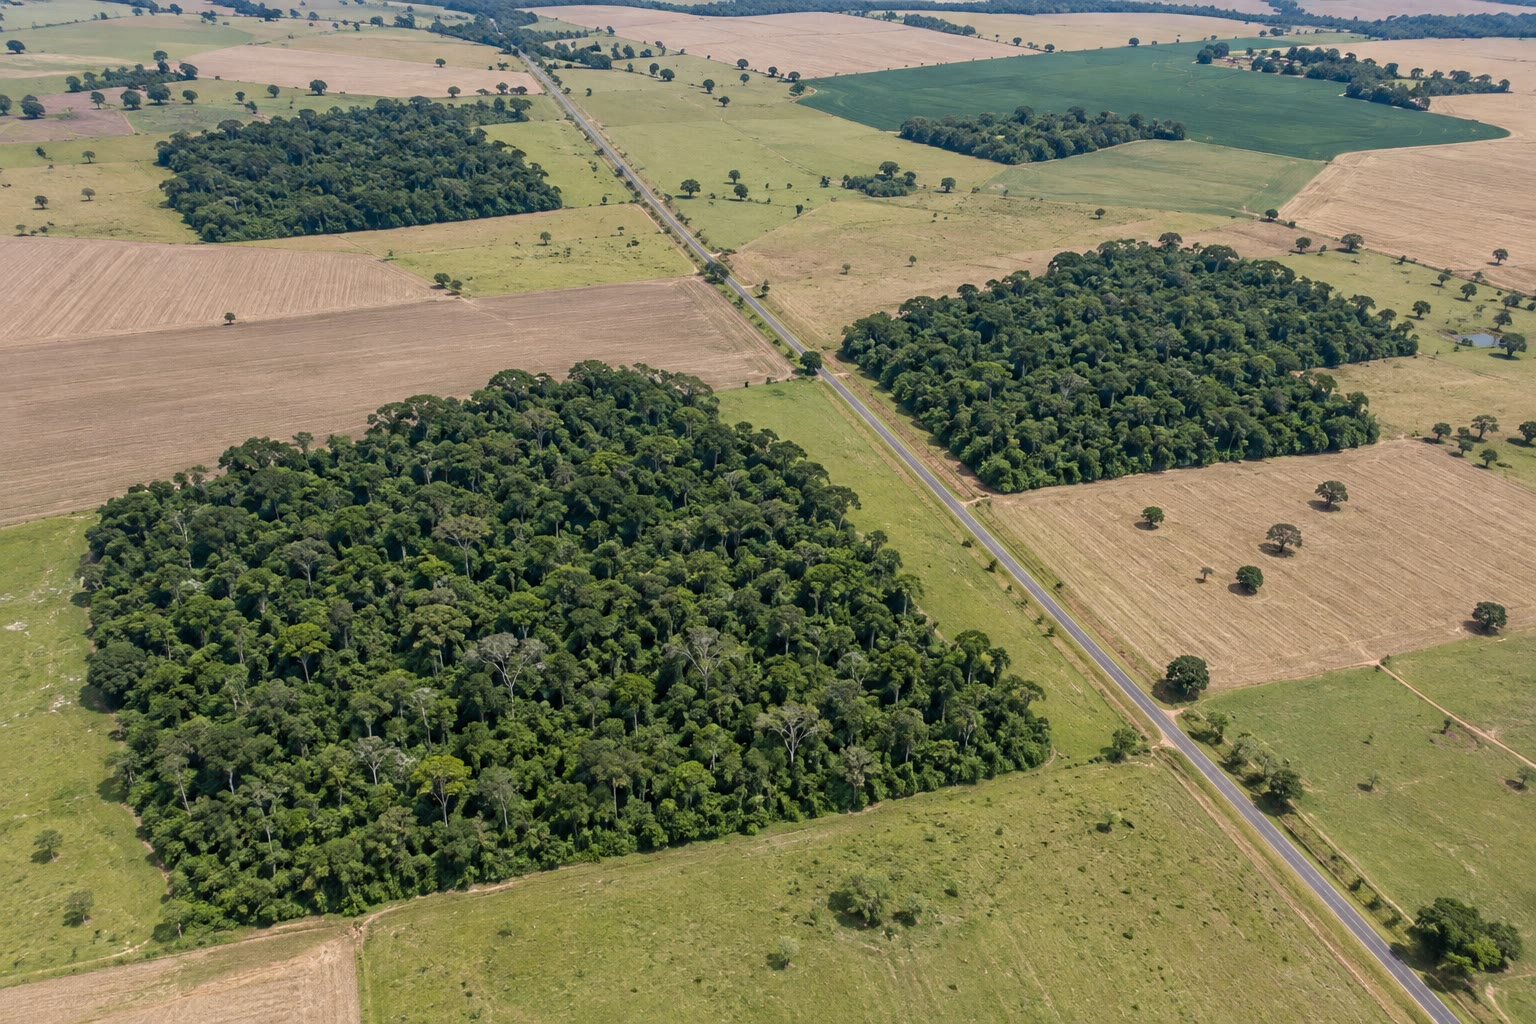
\includegraphics[width=0.6\linewidth]{images/book5/ai/b5-27-forest-fragments.jpg}

{\small Fragmentos de bosque entre campos de cultivo, vistos desde el
aire: cada isla alberga una población menor que la del conjunto,
bordeada por una franja que las especies del interior no pueden usar, y
separada por campos que las especies de bosque no pueden cruzar.}
\end{omfigure}

\section{Predecir y prevenir}

\begin{method}[El análisis de viabilidad poblacional]\label{met:b3:conservation-biology:pva}
\index{análisis de viabilidad poblacional}\index{cuasiextinción}
Para estimar el riesgo de extinción de una población y qué lo
reduciría: (1) constrúyase un modelo de su dinámica ---una matriz de
supervivencias y fecundidades por edad o por estadio, como en la
demografía del volumen del Año~2, estimada a partir de individuos
marcados a lo largo de varios años---; (2) añádase estocasticidad
---demográfica, sorteando al azar el destino de cada individuo, y
ambiental, sorteando las tasas de cada año a partir de su varianza
observada, con catástrofes ocasionales---; (3) añádanse la dependencia
de la densidad y el declive genético de la endogamia allí donde los
datos lo permitan; (4) simúlense miles de trayectorias desde el tamaño
actual a lo largo del horizonte de interés y regístrese la fracción que
cae por debajo de un umbral de \emph{cuasiextinción} (un tamaño desde
el cual se juzga imposible la recuperación); (5) váriense las entradas
---supervivencia adulta, supervivencia juvenil, área de hábitat, una
translocación de diez animales--- y véase qué cambio reduce más el
riesgo; ahí es donde debe ir el esfuerzo. La salida es una probabilidad
con una incertidumbre amplia, no una predicción; su valor es
comparativo, y ha mostrado una y otra vez que la palanca en las
especies longevas es la supervivencia adulta y no la fecundidad, por lo
que los palangres matan poblaciones de albatros que ponen un huevo cada
dos años más deprisa de lo que podría hacerlo cualquier pérdida de
nidos.
\end{method}

\begin{proposition}[El tiempo hasta la extinción]\label{prop:b3:conservation-biology:time}
\index{tiempo de extinción}
Para una población que fluctúa porque fluctúa el ambiente, con una tasa
media de crecimiento $\bar r$ cercana a cero y una varianza
$\sigma^{2}$ en la tasa anual de crecimiento, el logaritmo del tamaño
poblacional hace un paseo aleatorio con deriva, y el tiempo esperado
hasta la extinción desde un tamaño $N$ crece solo como el
\emph{logaritmo} de $N$ cuando $\bar r < 0$ ---duplicar la población
añade un número fijo de años--- y como una \emph{potencia} de $N$
cuando $\bar r > 0$, con exponente $2\bar r/\sigma^{2} - 1$; bajo la
sola \omterm{def:b3:conservation-biology:small}{estocasticidad demográfica} crece \emph{exponencialmente} con $N$,
de modo que una población a salvo del azar demográfico con cien
individuos puede perderse aún por la varianza ambiental con diez mil. La
consecuencia práctica es que reducir la varianza del crecimiento de una
población ---amortiguándola frente a los malos años con más hábitat,
más lugares, una dieta más amplia--- puede hacer más por su
persistencia que elevar su media.
\end{proposition}
\admitted

\begin{omfigure}
\begin{tikzpicture}
\begin{semilogyaxis}[
  width=0.62\linewidth, height=5.4cm,
  axis x line=bottom, axis y line=left,
  xmin=0, xmax=50, ymin=1, ymax=3000,
  xlabel={años}, ylabel={tamaño de la población},
  xlabel style={font=\small, at={(axis description cs:0.5,-0.12)}, anchor=north}, ylabel style={font=\small},
  tick label style={font=\small}, xtick={0,10,20,30,40,50}, ytick={1,10,100,1000}, yticklabels={1,10,100,1000},
  clip=false,
]
\addplot[thick, omDef] coordinates {(0,200) (2,240) (4,190) (6,260) (8,300) (10,220) (12,180) (14,250) (16,330) (18,280) (20,350) (22,300) (24,260) (26,340) (28,420) (30,380) (32,450) (34,400) (36,520) (38,480) (40,560) (42,500) (44,600) (46,650) (48,610) (50,700)};
\addplot[thick, omThm] coordinates {(0,200) (2,150) (4,180) (6,120) (8,90) (10,110) (12,70) (14,50) (16,60) (18,35) (20,40) (22,25) (24,18) (26,22) (28,12) (30,8) (32,9) (34,5) (36,3) (38,2) (40,1)};
\addplot[thick, omMeth!70!black] coordinates {(0,200) (2,210) (4,170) (6,200) (8,140) (10,160) (12,120) (14,140) (16,90) (18,110) (20,80) (22,95) (24,60) (26,75) (28,50) (30,55) (32,40) (34,45) (36,30) (38,35) (40,28) (42,30) (44,22) (46,25) (48,20) (50,22)};
\draw[dashed, gray] (axis cs:0,20) -- (axis cs:50,20); \node[font=\scriptsize, gray, anchor=north east] at (axis cs:49,18) {umbral de cuasiextinción};
\node[font=\scriptsize, omDef, anchor=west] at (axis cs:50.5,700) {$\bar r > 0$: persiste};
\node[font=\scriptsize, omMeth!70!black, anchor=west] at (axis cs:50.5,22) {$\bar r \approx 0$: a la deriva hacia abajo};
\node[font=\scriptsize, omThm, anchor=west] at (axis cs:40.5,1.3) {$\bar r < 0$: desaparecida en 40 años};
\end{semilogyaxis}
\end{tikzpicture}

{\small Tres trayectorias simuladas a partir de los mismos doscientos
animales, que difieren solo en la tasa media de crecimiento; un
análisis de viabilidad corre miles de ellas y cuenta cuántas cruzan el
umbral. La varianza de un año a otro es lo que convierte en una
apuesta incluso el caso intermedio.}
\end{omfigure}

\begin{definition}[Las herramientas]\label{def:b3:conservation-biology:tools}
\index{Lista Roja de la UICN}\index{especie invasora}\index{conservación ex situ}\index{cría en cautividad}\index{reintroducción}\index{renaturalización}\index{cascada trófica}
La \emph{Lista Roja de la UICN} clasifica las especies con criterios
cuantitativos: un declive del \qty{30}{\%}, del \qty{50}{\%} o del
\qty{80}{\%} en diez años o tres generaciones, un área de distribución
por debajo de \qty{20000}{}, \qty{5000}{} o \qty{100}{km^2}, una
población por debajo de \qty{10000}{}, \qty{2500}{} o \qty{250}{}
individuos maduros, o una probabilidad de extinción modelizada, sitúan
a una especie como Vulnerable, En Peligro o En Peligro Crítico; una
cuarta parte de los mamíferos y una octava de las aves lo cumplen. Las
causas son, primero, la pérdida de hábitat; después, la
sobreexplotación, las \emph{especies invasoras} (depredadores y
competidores llevados a islas cuyas especies nunca los habían
encontrado: las ratas, los gatos y los armiños se han llevado a la
mayoría de las aves de Nueva Zelanda, y una sola especie de serpiente
arbórea parda a la mayoría de las de Guam), la contaminación y el
cambio climático. Las respuestas: áreas protegidas que cubren la sexta
parte de la tierra firme; el control o la erradicación de los invasores
(ciento cincuenta islas libradas de ratas); la conservación \emph{ex
situ} ---bancos de semillas que guardan un millón de accesiones en una
cámara del permafrost ártico, embriones congelados y la \emph{cría en
cautividad} con genealogías gestionadas para minimizar el parentesco,
que devolvió al cóndor de California desde veintidós aves en 1987 y al
turón patinegro desde dieciocho---; la \emph{reintroducción}, que
funciona alrededor de un tercio de las veces, y más a menudo cuando se
ha eliminado la causa de la pérdida original; y la
\emph{renaturalización}, el retorno de los animales grandes y de los
procesos que impulsan ---los lobos de Yellowstone, cuya depredación y
cuyo miedo apartaron a los uapitíes de las riberas y dejaron volver al
sauce, al álamo, al castor y a las aves canoras, una \emph{cascada
trófica} que va de un carnívoro a la forma de un río.
\end{definition}

\begin{omfigure}
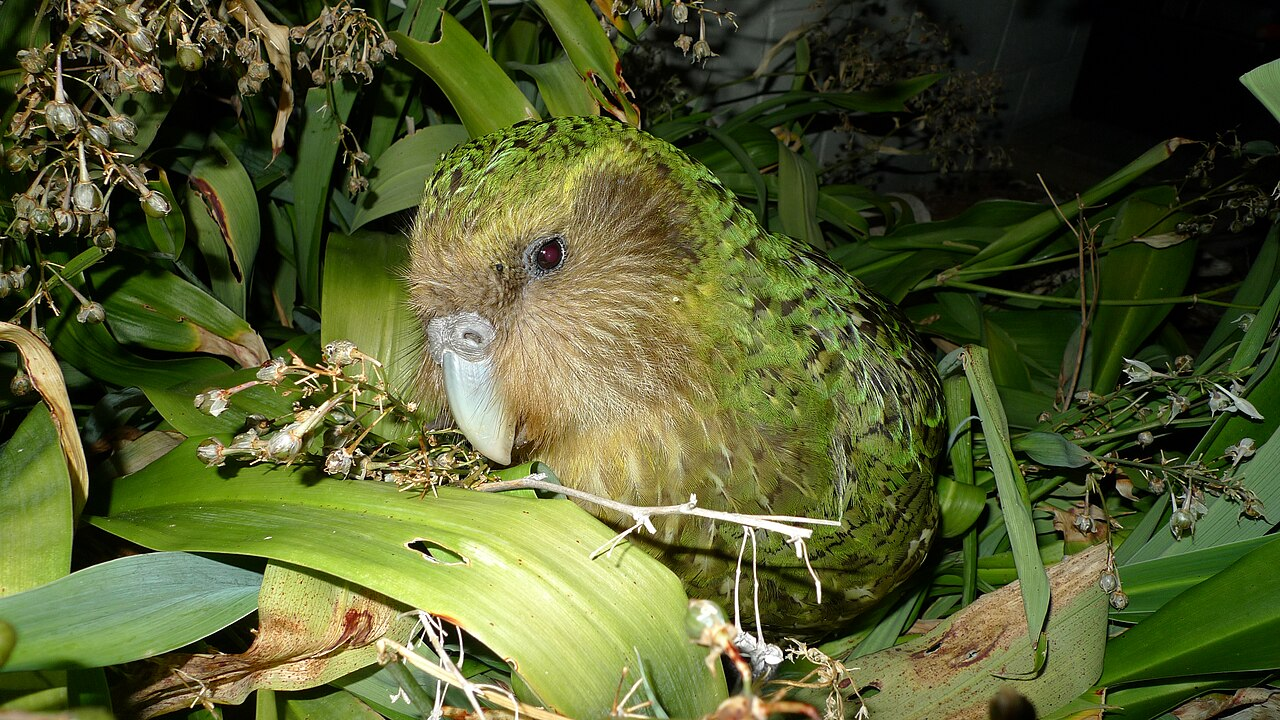
\includegraphics[width=0.46\linewidth]{images/book5/kakapo-sirocco.jpg}\hspace{0.04\linewidth}
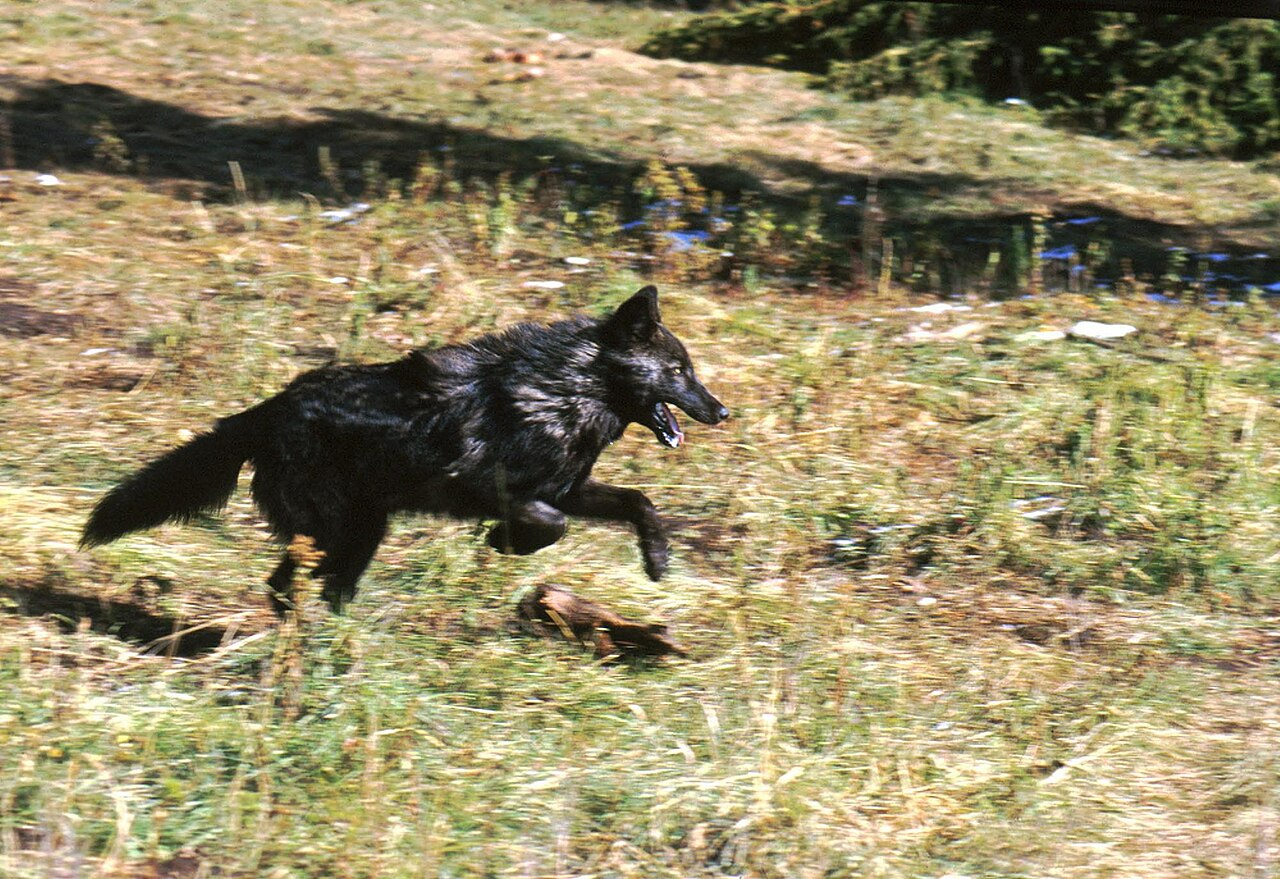
\includegraphics[width=0.46\linewidth]{images/book5/yellowstone-wolves-1996.jpg}

{\small Izquierda: Sirocco, un kakapo ---uno de los cincuenta y un
supervivientes de 1995, hoy uno de unos doscientos cincuenta, todos
bautizados y vigilados en islas libres de depredadores (fotografía:
Department of Conservation, Nueva Zelanda, CC BY 2.0). Derecha: lobos en
Yellowstone en 1996, el primer invierno tras su \omterm{def:b3:conservation-biology:tools}{reintroducción}
(fotografía: National Park Service, dominio público).}
\end{omfigure}

\begin{example}[Tres recuperaciones]\label{ex:b3:conservation-biology:recoveries}
El kakapo: cincuenta y un ejemplares en 1995, todos trasladados a islas
libradas de depredadores; cada ave lleva un transmisor, cada nido se
vigila con cámara, los pollos se crían a mano cuando una madre falla,
los machos reciben alimento suplementario para ponerlos en condición
reproductora los años en que fructifican los rimus, y la genealogía se
gestiona para conservar en la población los genes raros del último
macho de Fiordland; se ha secuenciado el genoma de todos los kakapos.
Ahora son doscientos cincuenta, con un $N_{e}$ que los genomas sitúan
cerca de cien. La grulla trompetera: quince aves en 1941, en una sola
bandada migratoria, criadas en cautividad a partir de huevos tomados de
nidos silvestres, enseñadas a seguir rutas migratorias nuevas tras
ultraligeros, y ahora unas ochocientas. La ballena jorobada: cazada
hasta unos pocos miles, protegida en 1966 y hoy por encima de cien mil,
con un aumento cercano al \qty{8}{\%} anual que muestra lo que hace un
animal longevo cuando se elimina la única causa de su declive. Cada
recuperación costó decenas de millones y décadas; la aritmética del
capítulo dice por qué hubo que gastar el esfuerzo antes de que los
números llegaran al vórtice, y por qué salió más barato que cualquier
rescate posterior.
\end{example}

\begin{omfigure}
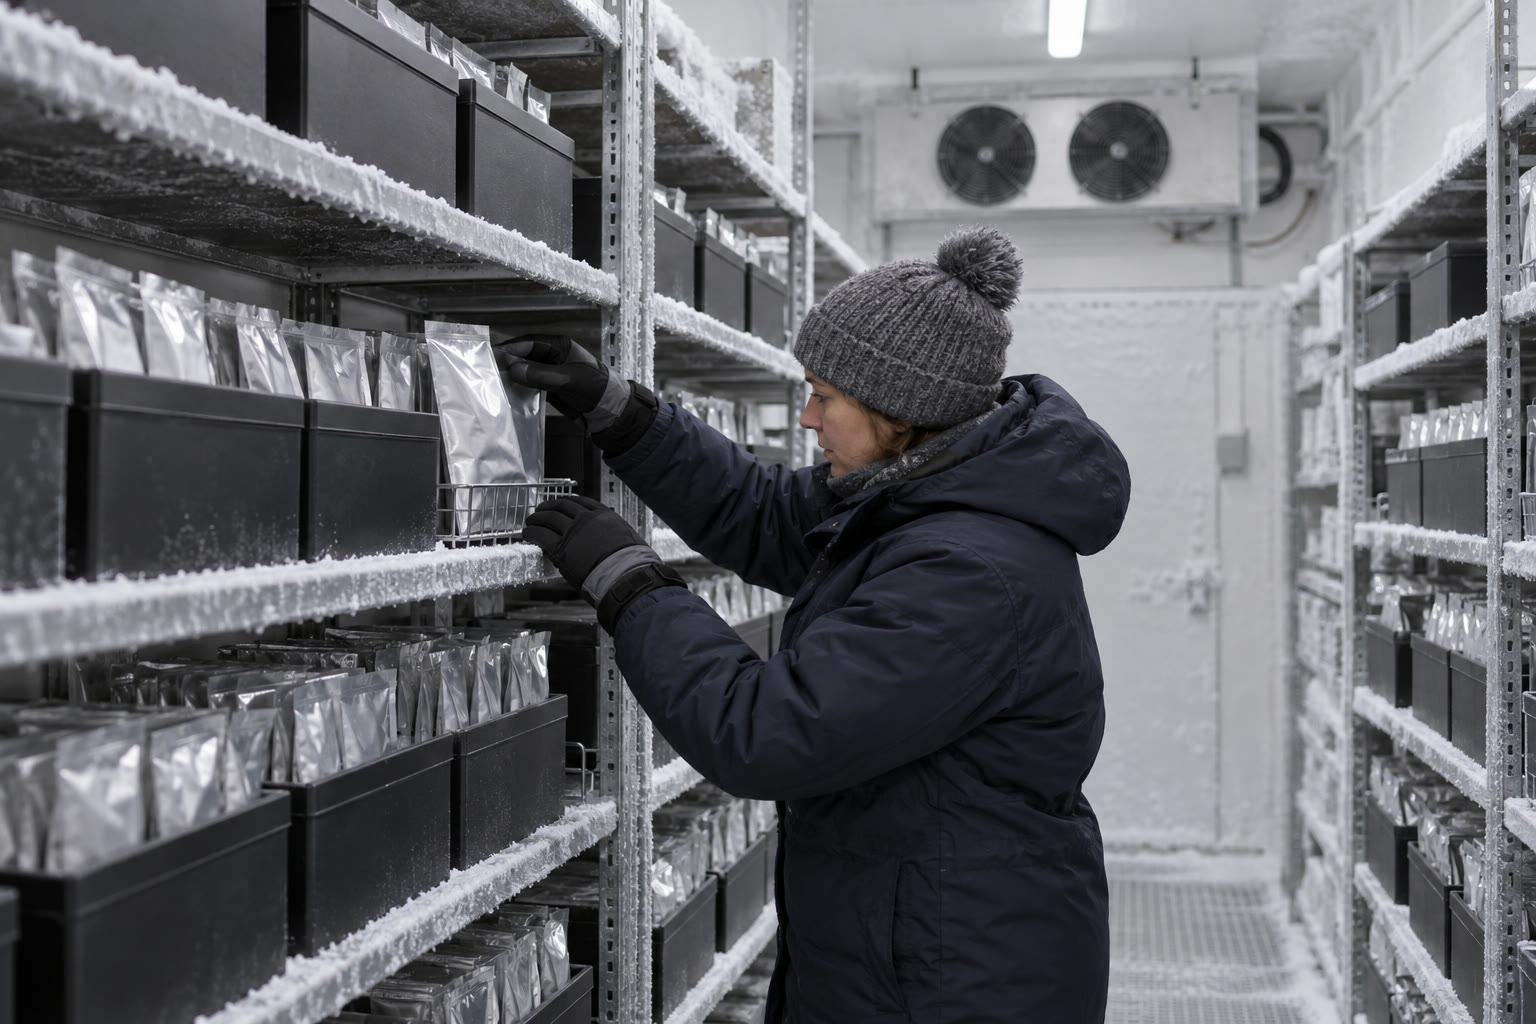
\includegraphics[width=0.56\linewidth]{images/book5/ai/b5-27-seed-vault.jpg}

{\small Una cámara de semillas en el permafrost: duplicados de un
millón de accesiones de cultivos y de plantas silvestres, conservadas a
\qty{-18}{\celsius} frente a la pérdida de las colecciones de las que
proceden ---la conservación como seguro, a la escala del genoma de una
especie.}
\end{omfigure}

\begin{remark}[La aritmética de conservar]\label{rem:b3:conservation-biology:remark}
Todos los capítulos de este curso han terminado en un número, y este
termina en varios: un tamaño efectivo, un \omterm{thm:b3:conservation-biology:ne}{coeficiente de endogamia} que
sube $1/2N_{e}$ por generación, un exponente $z$ que convierte las
hectáreas perdidas en especies perdidas, una probabilidad de extinción
en un siglo. Son burdos ---el censo es incierto, la varianza se
adivina, el modelo es una caricatura--- y son lo que convierte un
sentimiento sobre unas aves que desaparecen en una decisión sobre qué
cincuenta hectáreas comprar y qué ocho animales mover. La biología es
la misma biología que la del resto del libro: deriva, selección,
demografía, comportamiento, la dependencia de una población respecto de
su hábitat y la de un hábitat respecto de sus poblaciones. Lo único
nuevo es la urgencia, y el hecho de que el experimento se está
haciendo una sola vez, sin control, con las especies que quedan.
\end{remark}

\section{Ejercicios}

\begin{exercise}[$\star$]\label{exo:b3:conservation-biology:1}
Defínanse la \omterm{def:b3:conservation-biology:small}{estocasticidad demográfica}, la \omterm{def:b3:conservation-biology:small}{estocasticidad ambiental} y
el \omterm{def:b3:conservation-biology:small}{efecto Allee}, y dese un ejemplo de cada uno tomado del capítulo.
\end{exercise}

\begin{exercise}[$\star$]\label{exo:b3:conservation-biology:2}
¿Qué es el \omterm{thm:b3:conservation-biology:ne}{tamaño efectivo de población}, y qué tres rasgos de una
población real lo hacen menor que el censo?
\end{exercise}

\begin{exercise}[$\star$]\label{exo:b3:conservation-biology:3}
Enúnciese la ley especies--área. Si $z = 0.25$, ¿qué fracción de
especies conserva un hábitat tras perder la mitad de su área? ¿Y nueve
décimas partes? ¿Y noventa y nueve centésimas?
\end{exercise}

\begin{exercise}[$\star$]\label{exo:b3:conservation-biology:4}
Explíquese la regla 50/500, y de qué protege cada número.
\end{exercise}

\begin{exercise}[$\star\star$]\label{exo:b3:conservation-biology:5}
Una manada de 200 elefantes marinos tiene 8 machos y 120 hembras
reproductores. Calcúlense $N_{e}$ y la pérdida de heterocigosidad por
generación. ¿Cuántas generaciones hacen falta para perder una cuarta
parte de ella?
\end{exercise}

\begin{exercise}[$\star\star$]\label{exo:b3:conservation-biology:6}
Una población contó 1000, 1000, 20, 1000 y 1000 en cinco generaciones
sucesivas. Calcúlense $N_{e}$ en ese tramo y la heterocigosidad
retenida, y compárese con un tamaño constante de 1000.
\end{exercise}

\begin{exercise}[$\star\star$]\label{exo:b3:conservation-biology:7}
Veinticinco panteras de Florida con $N_{e} \approx 10$: ¿endogamia
acumulada en 5 generaciones? Si la eficacia cae un \qty{5}{\%} por cada
\qty{10}{\%} de $F$, ¿cuánto ha caído la eficacia? ¿Qué le hace a $F$ en
la generación siguiente añadir ocho hembras sin parentesco?
\end{exercise}

\begin{exercise}[$\star\star$]\label{exo:b3:conservation-biology:8}
Yellowstone: 31 lobos soltados en 1995--96 y alrededor de 100 en el
parque en 2003. Estímese $r$; ¿cuántos habría en 2020 si el crecimiento
hubiera continuado, y por qué no fue así?
\end{exercise}

\begin{exercise}[$\star\star$]\label{exo:b3:conservation-biology:9}
Clasifíquense con los criterios de la UICN del capítulo: (a) una rana
cuya población cayó un \qty{60}{\%} en diez años; (b) una planta de 180
individuos maduros; (c) un pez cuya área de distribución es de
\qty{3000}{km^2}; (d) un ave de \num{30000} individuos que declina un
\qty{10}{\%} por década.
\end{exercise}

\begin{exercise}[$\star\star\star$]\label{exo:b3:conservation-biology:10}
Una población de $N$ parejas que producen, con probabilidad $1/2$, dos
descendientes supervivientes y en caso contrario ninguno
(\omterm{def:b3:conservation-biology:small}{estocasticidad demográfica}). Calcúlese la probabilidad de que toda la
población fracase en una generación para $N = 2$, $5$, $10$ y $20$, y
coméntese cómo escala el riesgo demográfico con $N$.
\end{exercise}

\begin{exercise}[$\star\star\star$]\label{exo:b3:conservation-biology:11}
La ley especies--área con $z = 0.25$, y un bosque cortado en 10
fragmentos aislados iguales. Compárense las especies esperadas en un
fragmento con las de una décima parte del original, y arguméntese por
qué el total de todos los fragmentos no es sencillamente el original:
¿qué determina que los fragmentos juntos alberguen más o menos especies
que el conjunto?
\end{exercise}

\begin{exercise}[$\star\star\star$]\label{exo:b3:conservation-biology:12}
¿Por qué añadir unos pocos migrantes por generación ($m N_{e} \approx 1$)
detiene en buena medida la pérdida de variación en una población
pequeña, y qué cuesta eso en adaptación local? Arguméntese con el
equilibrio entre la deriva, $1/2N_{e}$, y la fracción de alelos
reemplazados por los migrantes, $m$.
\end{exercise}

\section{Problema: cincuenta y quinientos}

\begin{problem}[{Problema de fin de semana --- un programa de
recuperación en números: el tamaño efectivo de una población rescatada
de loros y su endogamia, un rescate genético, las especies que
conservará un bosque que encoge, el crecimiento de unos lobos
reintroducidos, y las categorías y los costes, para terminar en
$N_{e}$, la endogamia tras diez generaciones y la fracción de especies
conservada}]
\label{pb:b3:conservation-biology:1}
Datos: una población de loros de 60 adultos, 20 machos y 40 hembras,
todos reproductores; tiempo de generación \qty{10}{yr}. Historia de la
población en las últimas cinco generaciones: 500, 100, 60, 51, 60.
Depresión por endogamia: la eficacia cae un \qty{6}{\%} por cada
\qty{0.1}{} de $F$. Rescate: 10 aves sin parentesco añadidas a las 60.
Bosque: \qty{2000}{km^2} reducidos a \qty{300}{km^2}, con $z = 0.25$;
180 especies ahora. Lobos: 31 soltados, 100 al cabo de 8 años,
capacidad de carga del parque de unos 120. Coste: cuatro millones de
dólares al año para los loros.

\medskip
\noindent\textbf{Parte I --- El tamaño efectivo.}
\begin{enumerate}
  \item $N_{e}$ a partir de la \omterm{thm:b3:conservation-biology:ne}{proporción de sexos} de los 60 actuales.
        Compárese con el censo.
  \item $N_{e}$ como \omterm{thm:b3:conservation-biology:ne}{media armónica} a lo largo de las cinco generaciones
        de historia. ¿Qué generación domina?
  \item Endogamia acumulada en esas cinco generaciones, usando el
        $N_{e}$ de \omterm{thm:b3:conservation-biology:ne}{media armónica} (fórmula exacta y aproximación
        lineal).
  \item Eficacia perdida por esa endogamia.
  \item Heterocigosidad retenida tras las cinco generaciones, como
        fracción de la original.
  \item Si la población se mantiene ahora en 60 con la \omterm{thm:b3:conservation-biology:ne}{proporción de
        sexos} actual, ¿qué $F$ alcanzará en diez generaciones más, y qué
        pérdida de eficacia? ¿Cuántos años son?
\end{enumerate}

\medskip
\noindent\textbf{Parte II --- El rescate.}
\begin{enumerate}[resume]
  \item Diez aves sin parentesco se suman a las 60. La fracción de
        alelos de la generación siguiente procedente de las recién
        llegadas es de alrededor de $10/70$; el \omterm{thm:b3:conservation-biology:ne}{coeficiente de endogamia}
        de la descendencia con un progenitor nativo y otro recién
        llegado es $0$. Estímese el $F$ medio de la población en la
        generación siguiente si el apareamiento es aleatorio.
  \item Explíquese por qué $F$ cae de inmediato pero la heterocigosidad
        solo sube a medida que se extienden los alelos de los migrantes,
        y por qué puede hacer falta un segundo rescate.
  \item Para alcanzar $N_{e} = 500$ con una \omterm{thm:b3:conservation-biology:ne}{proporción de sexos} igual,
        ¿cuántos adultos hacen falta? A $r = \qty{0.05}{yr^{-1}}$ desde
        70 aves, ¿cuántos años?
  \item El programa retira huevos de las malas madres para criarlos a
        mano, lo que eleva el número medio de pollos volanderos por
        pareja pero iguala los tamaños de familia. ¿Por qué igualar los
        tamaños de familia \emph{eleva} $N_{e}$ por encima del censo
        (hacia $2N$)?
  \item El último macho de un linaje meridional distinto es estéril en
        libertad. Propónganse dos intervenciones y sus costes para el
        acervo génico.
  \item A cuatro millones de dólares al año a lo largo de los 40 años
        necesarios para alcanzar $N_{e} = 500$, coste total y coste por
        ave añadida. ¿Es caro? ¿Frente a qué?
\end{enumerate}

\medskip
\noindent\textbf{Parte III --- El bosque.}
\begin{enumerate}[resume]
  \item Fracción de especies que conservará el bosque con
        \qty{300}{km^2}; número esperado de especies y deuda de
        extinción (especies presentes ahora que se perderán).
  \item Si en cambio los \qty{300}{km^2} fueran tres fragmentos
        aislados de \qty{100}{km^2}, especies por fragmento; total si
        los fragmentos albergaran especies enteramente distintas; total
        si albergaran las mismas. ¿Qué lo decide?
  \item Un corredor de \qty{20}{km^2} une los tres fragmentos.
        Trátense como una sola área de \qty{320}{km^2}: especies
        esperadas. Compárese con el caso de especies idénticas de la
        pregunta~14.
  \item El mayor depredador del bosque necesita \qty{50}{km^2} por
        pareja y un $N_{e}$ de 50 para persistir. ¿Pueden albergarlo los
        \qty{300}{km^2} enteros? ¿Y un fragmento? ¿Qué dice esto sobre
        el área frente al número de especies como criterio?
  \item Estímese cuánto tarda en pagarse la deuda de extinción si las
        especies perdidas tienen poblaciones que declinan un \qty{3}{\%}
        anual desde 200 hasta un umbral de cuasiextinción de 10.
  \item ¿Por qué la ley especies--área subestima la pérdida cuando la
        fragmentación añade \omterm{prop:b3:conservation-biology:area}{efectos de borde}, y la sobreestima cuando el
        terreno circundante es en parte utilizable?
\end{enumerate}

\medskip
\noindent\textbf{Parte IV --- Lobos y listas.}
\begin{enumerate}[resume]
  \item Lobos: $r$ a partir de $31 \to 100$ en 8 años, y el tiempo de
        duplicación.
  \item Crecimiento logístico hacia $K = 120$: población tras 8 años con
        crecimiento logístico en lugar de exponencial, partiendo de 31
        con la $r$ de la pregunta~19 (úsese $N(t) = K/[1 + (K/N_{0} -
        1)\mathrm{e}^{-rt}]$). ¿Cuál se ajusta mejor a los 100
        observados, y qué dice eso sobre la dependencia de la densidad
        en los primeros años?
  \item Los uapitíes eran \num{17000} en 1995 y \num{4000} en 2015.
        Tasa media anual de declive. ¿Qué parte de ella pueden explicar
        unos lobos que comen \num{20} uapitíes cada uno al año, con 100
        lobos?
  \item Clasifíquense el loro (60 individuos maduros) y el depredador
        del bosque antes del rescate con los criterios de la UICN.
  \item Paloma migratoria: cinco mil millones en 1800, extinta en 1914.
        Si el declive fue exponencial desde 1870, cuando todavía había
        miles de millones, hasta un ave en 1914, ¿qué tasa anual implica
        eso? ¿Por qué el \omterm{def:b3:conservation-biology:small}{efecto Allee} hace las últimas décadas más
        rápidas que una exponencial?
  \item Explíquese en un párrafo por qué un análisis de viabilidad
        habría dicho que la paloma migratoria estaba a salvo en 1850, y
        qué se le habría escapado.
  \item Resúmase: el $N_{e}$ actual (pregunta~1), $F$ tras diez
        generaciones más con 60 individuos (pregunta~6) y la fracción de
        especies que conserva el bosque encogido (pregunta~13).
\end{enumerate}
\end{problem}
